%\documentclass{ximera}
\documentclass[handout,space,nooutcomes]{ximera}

\graphicspath{{./}{eulerCharacteristic}}


\title{Paying off Debt, Part 2}
\author{Brad Findell \and Bart Snapp}
\begin{document}
\begin{abstract}
Here we continue to investigate where your payments go when you pay off debt.
\end{abstract}
\maketitle

\begin{question}[1in]
Suppose you borrow $\$P$ and agree to pay it back in equal annual
payments over $7$ years, with an annual interest rate of $r$, compounded annually.  

\begin{itemize}
\item Call the annual payment $x$.
\item Use the table from last week's class, showing the interest, payment, and remaining
principal at the end of years $1, 2, 3, \dots$.  
\item Collect factors of $(1+r)$ where you can.  
\item Let $P_n$ denote the principal in year $n$, with $P_0=P$, and write a recursive formula for $P_n$ in terms of $P_{n-1}$, $r$, and $x$ for $n\ge 1$.  
\end{itemize}

%\[
%\answer{P(1+r)^5-x(1+r)^4 -x(1+r)^3-x(1+r)^2 - x(1+r) -x} = 0.
%\]


%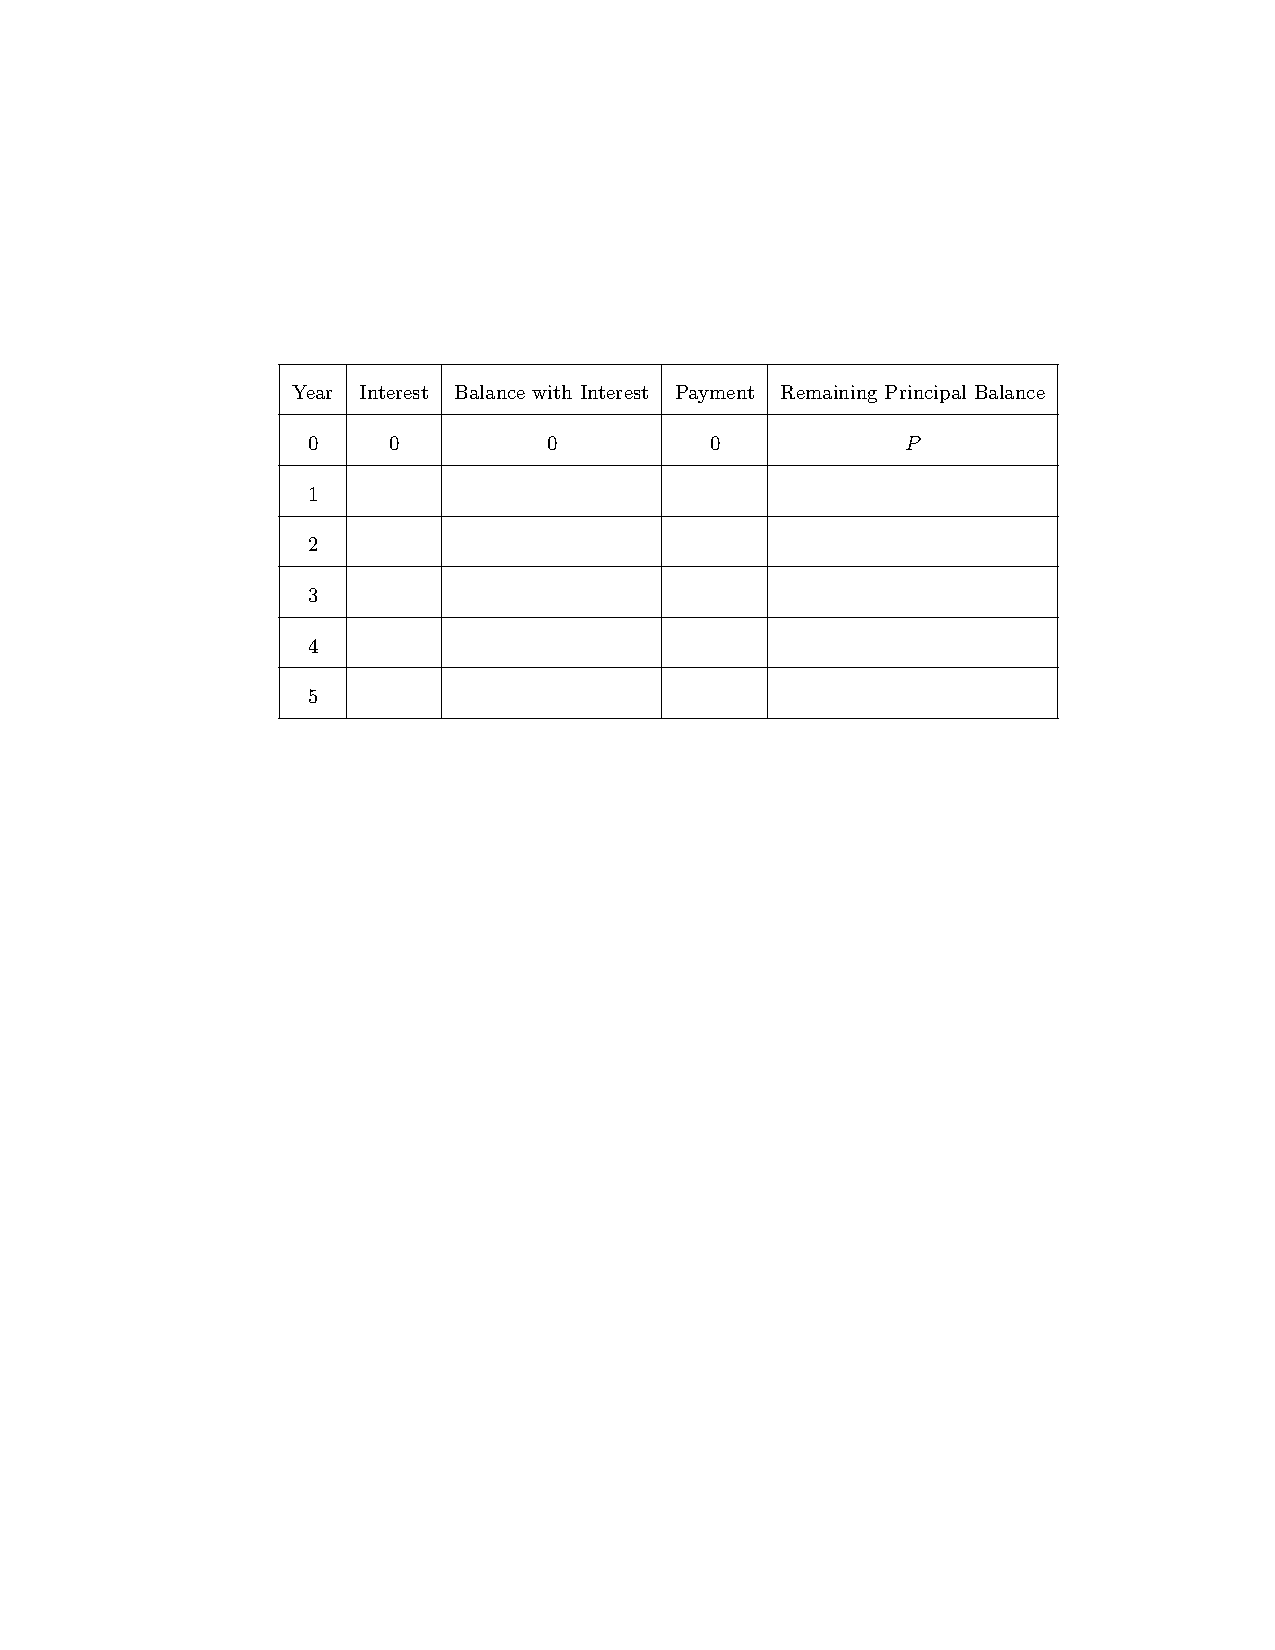
\includegraphics[scale=1.2]{payingOffDebtTableGraphic2.pdf}

\def\arraystretch{3}
\begin{table}[h]
\begin{tabular}{|c|c|c|c|l|}
\hline
Year, $n$ & Accumulated Interest & Balance with Interest & Payment & Remaining Principal Balance, $P_n$ \\ \hline
0    &   ---    &       ---          &   ---   &  $P_0=P$               \\ \hline
1    &          &                    &         &  $P_1=$                 \\ \hline
2    &          &                    &         &  $P_2=$                  \\ \hline
3    &          &                    &         &  $P_3=$                  \\ \hline
\end{tabular}
\end{table}
\vfill
So $P_n = $
\vfill
\end{question}
\newpage
\begin{question}
As a step toward a closed formula for $P_n$, write out expressions for $P_1$, $P_2$, $P_3$, \dots in terms of $P$, $r$, and $x$, and try to find a pattern (using dots).  
\begin{freeResponse}
\end{freeResponse}
\vfill
\end{question}


\newpage

\begin{question}
Some students notice that the equation above includes a geometric
series.  Which of the following are examples of geometric series?
\begin{multipleChoice}
  \choice{$1+2+3+4+5+6+7$}
  \choice[correct]{$(1/2) + (1/2)^2 + (1/2)^3 + (1/2)^4+(1/2)^5$}
  \choice{$3+6+9+12+15+18+21$}
  \choice[correct]{$(1+r) + (1+r)^2 + (1+r)^3 + (1+r)^4+ (1+r)^5$}
  \choice[correct]{$0.151515151515\dots$}
\end{multipleChoice}

\end{question}




\begin{question}
Find a closed-form expression for the sum of the geometric series:
  \[
  1 + (1+r) + (1+r)^2 + (1+r)^3 + \dots + (1+r)^{n-2}+ (1+r)^{n-1}
  \]
  \[
  \answer{\frac{(1+r)^n-1}{r}}
  \]
Hint: Call the geometric series $S$, and note that if you multiply $S$ by the ``common ratio,'' you get another geometric series with many of the same terms.  Use these observations to find the sum of the series.   
\begin{freeResponse}
\end{freeResponse}
  \vfill
\end{question}


\newpage

 \begin{question}
 Use the closed-form expression for the sum of the geometric series to solve your equation for $x$, the annual payment.   
 \begin{freeResponse}
 \end{freeResponse}
 \vfill
 \end{question}
\newpage 

\begin{question}
What about monthly payments?  In other words, suppose you borrow $\$P$ and agree to pay it back in equal monthly
payments over $n$ years, with an annual interest rate of $r$, compounded monthly.  
Write a formula for the monthly payment.  
\begin{freeResponse}
\end{freeResponse}
\vfill
\end{question}

%Now let's use your formula!  
%
%\begin{question}
%Suppose that you buy a house with a $\$120,000$ mortgage, to be
%paid back in equal monthly payments over $30$ years.  If the interest
%rate is $6\%$, compounded monthly, what is your monthly payment? $\answer{719.46}$
%\begin{freeResponse}
%\end{freeResponse}
%\vfill
%\end{question}
%
%\break
%
%\begin{question}
%For this $\$120,000$ mortgage, how much interest and how much principal
%would you pay in the first month?  
%
%Interest: $\answer{600}$
%Principal:  $\answer{119.46}$
%\end{question}
%
%\begin{question}
%For the same mortgage, how much interest would you pay in total over the $30$ years?
%$\answer{139005.60}$
%\end{question}

%\begin{question}
%Finding an equal monthly payment for paying off a debt is a foundational problem in financial mathematics.  
%How might this problem change for more complicated financial transactions?  Consider the perspectives of 
%borrowers, lenders, bankers, investors, etc.  
%\begin{freeResponse}
%\end{freeResponse}
%\end{question}

\end{document}
